% ----------------------------------------------------------------
% AMS-LaTeX Paper ************************************************
% **** -----------------------------------------------------------
\documentclass[10pt]{amsart}
%\textwidth 14.5cm
%\textheight 22cm
%\hoffset -1.5cm
%\voffset -2.2cm
\usepackage{graphicx}
\usepackage{latexsym}
\usepackage{amsfonts}
\usepackage{amsthm}
\usepackage{amssymb}
\usepackage{amsmath}
\usepackage{enumerate}
\usepackage{color}
\usepackage{stmaryrd}
\usepackage{chemarrow}
\usepackage[all]{xy}
\usepackage[pdftex,bookmarksnumbered,bookmarksopen,colorlinks,linkcolor=blue,anchorcolor=black,citecolor=blue,urlcolor=blue]{hyperref}
\usepackage{booktabs}
\usepackage{subfigure}
\usepackage{makecell}

%\usepackage{mathabx}
% ----------------------------------------------------------------
\vfuzz2pt % Don't report over-full v-boxes if over-edge is small
\hfuzz2pt % Don't report over-full h-boxes if over-edge is small
% THEOREMS -------------------------------------------------------
\newtheorem{thm}{Theorem}[section]
\newtheorem{cor}[thm]{Corollary}
\newtheorem{lem}[thm]{Lemma}
\newtheorem{prop}[thm]{Proposition}
\theoremstyle{definition}
\newtheorem{defn}[thm]{Definition}
\theoremstyle{remark}
\newtheorem{rem}[thm]{Remark}
%\numberwithin{equation}{section}
% MATH -----------------------------------------------------------
\newcommand{\norm}[1]{\left\Vert#1\right\Vert}
\newcommand{\abs}[1]{\left\vert#1\right\vert}
\newcommand{\set}[1]{\left\{#1\right\}}
\newcommand{\Real}{\mathbb R}
\newcommand{\eps}{\varepsilon}
\newcommand{\To}{\longrightarrow}
\newcommand{\BX}{\mathbf{B}(X)}
\newcommand{\A}{\mathcal{A}}

\newcommand{\dx}{\,{\rm d}x}
\newcommand{\dd}{\,{\rm d}}
\newcommand{\bs}{\boldsymbol}
\newcommand{\mcal}{\mathcal}

\DeclareMathOperator*{\img}{img}
%\DeclareMathOperator*{\span}{span}
\newcommand{\sign}{\operatorname{sign}}
\newcommand{\curl}{\operatorname{curl}}
\renewcommand{\div}{\operatorname{div}}
%\renewcommand{\grad}{\operatorname{grad}}
\newcommand{\grad}{\operatorname{grad}}
\newcommand{\tr}{\operatorname{tr}}
% \DeclareMathOperator*{\tr}{tr}
\DeclareMathOperator*{\rot}{rot}
\DeclareMathOperator*{\var}{Var}
\newcommand{\dev}{\operatorname{dev}}
\newcommand{\sym}{\operatorname{sym}}
\newcommand{\skw}{\operatorname{skw}}
\newcommand{\spn}{\operatorname{spn}}
\newcommand{\mspn}{\operatorname{mspn}}
\newcommand{\mskw}{\operatorname{mskw}}
\newcommand{\vskw}{\operatorname{vskw}}
\newcommand{\vspn}{\operatorname{vspn}}
\newcommand{\defm}{\operatorname{def}}
\newcommand{\hess}{\operatorname{hess}}
% ----------------------------------------------------------------
\begin{document}

\title{\large Detailed Response to Referees}%

\date{}%
%\dedicatory{}%
%\commby{}%
% ----------------------------------------------------------------

\maketitle

The authors greatly appreciate the questions and concerns the reviewers have raised in the reports, as well as the careful reading. 
We have revised our manuscript in terms of your suggestions and polished the writing throughout. 
Other than some single word typos, important changes are highlighted in colored texts in this revision. 



\tableofcontents

%We thank the Referee for the valuable comments that helped us to improve the manuscript. In
%the revised version of the manuscript, all non-minor modifications are highlighted in red colour.
%Below, we address the points raised in the report.

\vskip0.5cm
\section{Response to Reviewer 1}
\begin{enumerate}[1.]

\item \textsf{The English presentation is unfortunately very dodgy and should be revised before any type of resubmission.}

\smallskip \noindent \textcolor[rgb]{1.00,0.00,0.00}{Reply.}
We try our best to proofread the manuscript carefully.


\medskip

\item \textsf{An important question is whether you have in mind specific occasions where stabilization free virtual elements are superior to stabilized ones. More precisely, your procedure is sensibly more expensive and complicated than that of the standard VEM: you need a simplicial tessellation of each element; you project on BDM-type polynomial spaces; the theoretical setting itself is rather involved. If there are no apparent advantages in some specific occasion, the stabilization-free approach seems to be rather lame.}

\smallskip \noindent \textcolor[rgb]{1.00,0.00,0.00}{Reply.}
The stabilization term in virtual element methods (VEM) brings about some problems, which motivate us to develop stabilization-free VEMs. 
\begin{enumerate}
\item 
The local stabilization term $S_K(\cdot, \cdot)$ has to satisfy 
$$
c_{*} |v|_{1,K}^2\leq S_K(v,v)\leq c^{*} |v|_{1,K}^2 
$$
for $v$ belongs to the non-polynomial subspace of the virtual element space, which influences the condition number of the stiffness matrix and brings in the pollution factor $\frac{\max\{1, c^*\}}{\min\{1, c_*\}}$ in the error estimates \cite{DassiMascotto2018,BeiraodaVeigaDassiRusso2017,Mascotto2018}.  
\item 
The stabilization term appears in both sides of the a posteriori error estimates when bounding the error by the residual error estimators \cite{CangianiGeorgoulisPryerSutton2017}.
\item 
For the a posteriori error analysis on anisotropic polygonal meshes in \cite{AntoniettiBerroneBorioDAuriaEtAl2022}, the stabilization dominates the error estimator, which makes the anisotropic a posteriori error estimator suboptimal. 
\item The stabilization term significantly affects the performance of the VEM for the Poisson eigenvalue problem \cite{BoffiGardiniGastaldi2020},
and improper choices of the stabilization term will produce useless results.
\item 
Special stabilization terms are designed for a nonlinear elasto-plastic deformation problem \cite{HudobivnikAldakheelWriggers2019} and an electromagnetic interface problem in three dimensions \cite{CaoChenGuo2023}, which are not easy to be extended to other problems.
\item Numerical examples in \cite{BerroneBorioMarcon2022} show that the stabilization-free VEM in \cite{BerroneBorioMarcon2021} outperforms the standard VEM in \cite{BeiraodaVeigaBrezziMariniRusso2016} for anisotropic elliptic problems on general convex polygonal meshes.
\end{enumerate}





\medskip

\item \textsf{Lines 17-18; when you discuss the results in references \cite{BerroneBorioMarcon2021,BerroneBorioMarcon2022,DAltriMirandaPatrunoSacco2021}, I am not quite sure that the polynomial degree of the projection depends only on the number of vertices. In fact, in an updated version of the preprint \cite{BerroneBorioMarcon2021}, it is possible to see that also the shape of the polygon plays a role in the choice of such a polynomial degree.}

\smallskip \noindent \textcolor[rgb]{1.00,0.00,0.00}{Reply.}
Yes. In \cite{BerroneBorioMarcon2021}, the polynomial degree $l$ should satisfy
$$
(l+1)(l+2) - \dim\mathcal{P}_l^{\textrm{ker}}(E)\geq N_E^V-1.
$$
And the dimension of $\mathcal{P}_l^{\textrm{ker}}(E)$ generally depends on the geometry of the polygon. While the authors prove that
$$
\dim\mathcal{P}_l^{\textrm{ker}}(E)\leq l(l+1)
$$
in \cite[Theorem 2]{BerroneBorioMarcon2021}. This means that a sufficient condition for $l$ is 
$$
l\geq \frac{1}{2}(N_E^V-3).
$$

\medskip

\item \textsf{Line 22; ``arbitrary dimension'' only refers to the nonconforming version of the scheme. Please, better highlight this fact.}

\smallskip \noindent \textcolor[rgb]{1.00,0.00,0.00}{Reply.}
Thanks for this suggestion. We have emphasized it.

\medskip

\item \textsf{I appreciate the fact that you “preview” equation (1.1) in the introduction, as it is the lynchpin of the forthcoming analysis. Yet, it would be beneficial a brief comment on the hidden constants. For instance, you should state on what such constants depend on.}

\smallskip \noindent \textcolor[rgb]{1.00,0.00,0.00}{Reply.}
Thanks for this suggestion. We have presented a comment as follows: The hidden constants in (1.1) are independent of the size of $K$, but depend on the degree of polynomials, and the chunkiness parameter and the geometric dimension of $K$; see Section~2.2 for details.

\medskip

\item \textsf{Lines 41-43; you should underline that the polynomial spaces onto which you project are based on a regular simplicial tessellation of the elements of the mesh.}

\smallskip \noindent \textcolor[rgb]{1.00,0.00,0.00}{Reply.}
Thanks for this suggestion. We have mentioned it.


\medskip

\item \textsf{Lines 50-51; when you define the function $\phi$, are you sure that the normal component of the trace is a polynomial only on the faces of $K$? Don't you also need this property to be valid on the faces of the simplicial tessellation of $K$?}

\smallskip \noindent \textcolor[rgb]{1.00,0.00,0.00}{Reply.}
Base on a $d$-dimensional polytope $K\in \mathcal T_h$ and its simplicial partition $\mathcal T_K$ of $K$, we define the following $H(\div)$-conforming finite element spaces in this paper:
% For $d$-dimensional polytope $K\in \mathcal T_h$ and $k\geq2$, let 
\begin{align*}    
\boldsymbol{V}_{k-1}^{\mathrm{BDM}}(K)&=\{\boldsymbol{\phi}\in\boldsymbol{H}(\div, K): \boldsymbol{\phi}|_{T}\in \mathbb P_{k-1}(T;\mathbb R^d) \textrm{ for each } T\in\mathcal T_K\}\textrm{ for } k\geq2, \\
\boldsymbol{V}^{\mathrm{RT}}(K)&=\{\boldsymbol{\phi}\in\boldsymbol{H}(\div, K): \boldsymbol{\phi}|_{T}\in \mathbb P_{0}(T;\mathbb R^d)+\boldsymbol{x}\mathbb P_{0}(T) \textrm{ for each } T\in\mathcal T_K\}, \\
\boldsymbol{V}_{k-1}^{\rm div}(K)&=\{\boldsymbol{\phi}\in\boldsymbol{V}_{k-1}^{\mathrm{BDM}}(K): \div\boldsymbol{\phi}\in\mathbb P_{k-2}(K)\}\textrm{ for } k\geq2, \\
\boldsymbol{V}_{0}^{\rm div}(K)&=\{\boldsymbol{\phi}\in\boldsymbol{V}_{0}^{\mathrm{RT}}(K): \div\boldsymbol{\phi}\in\mathbb P_{0}(K)\},
\\
\mathbb{V}_{k-1}^{\rm div}(K)&=\{\boldsymbol{\phi}\in\boldsymbol{V}_{k-1}^{\rm div}(K): \boldsymbol{\phi}\cdot\boldsymbol{n}|_F\in\mathbb P_{k-1}(F) \textrm{ for each } F\in\mathcal F(K)\}.
\end{align*}
We compare these spaces for polytope $K$ and face $F\in\mathcal F(K)$ in the following table.
\begin{center}
\renewcommand\arraystretch{1.3}
\begin{tabular}[t]{|c|c|c|c|}
% \toprule
\hline
$\boldsymbol{\phi}$ & $\boldsymbol{V}_{k-1}^{\mathrm{BDM}}(K)/\boldsymbol{V}^{\mathrm{RT}}(K)$ & $\boldsymbol{V}_{k-1}^{\rm div}(K)$ & $\mathbb{V}_{k-1}^{\rm div}(K)$  \\
\hline
% \midrule 
$(\div\boldsymbol{\phi})|_K$ & piecewise polynomial & polynomial & polynomial \\
\hline
$(\boldsymbol{\phi}\cdot\boldsymbol{n})|_F$ & piecewise polynomial & piecewise polynomial & polynomial \\
\hline
% \bottomrule
\end{tabular}
\end{center}
We can see that both $(\div\boldsymbol{\phi})|_K$ and $(\boldsymbol{\phi}\cdot\boldsymbol{n})|_F$ are polynomials for $\boldsymbol{\phi}\in\mathbb{V}_{k-1}^{\rm div}(K)$.

To ensure the $L^2$ projection
$Q_{K,k}^{\div}\nabla v$ onto the space $\mathbb{V}_{k}^{\rm div}(K)$ is computable
for virtual element function $v\in V_k(K)$, we only require
$(\boldsymbol{\phi}\cdot\boldsymbol{n})|_F$ to be a polynomial for each $(d-1)$-dimensional face $F$ of $K$. But $(\boldsymbol{\phi}\cdot\boldsymbol{n})|_F$ can be a piecewise polynomial for interior face $F$ of the simplicial tessellation of $K$.


\medskip

\item \textsf{Line 138; you may wish to recall the degrees of freedom of this space, even though they are well known.}

\smallskip \noindent \textcolor[rgb]{1.00,0.00,0.00}{Reply.}
Thanks for this suggestion. We have recalled it.


\medskip

\item \textsf{Line 305; reference [21, Lemma 10] for the polynomial inverse inequality is not proper; in fact, the inverse estimate follows from standard polynomial inverse estimates on simplices (refer, e.g., to Verf{\"u}rth's book), the regularity of the element, and standard polynomial inverse estimates.}

\smallskip \noindent \textcolor[rgb]{1.00,0.00,0.00}{Reply.}
We add references \cite{Ciarlet1978,Verfuerth2013} in the revised manuscript.

\medskip

\item \textsf{Line 305; reference [11, (2.18)] is also a standard scaled trace inequality (refer to any PDE textbook).}

\smallskip \noindent \textcolor[rgb]{1.00,0.00,0.00}{Reply.}
We add reference \cite[Theorem 1.5.1.10]{Grisvard1985} in the revised manuscript.

\medskip

\item \textsf{Line 308-309; you also use the definition of negative norm (which I cannot find), an integration by parts, and a Cauchy-Schwarz inequality.}

\smallskip \noindent \textcolor[rgb]{1.00,0.00,0.00}{Reply.}
We revise the first part of the proof of Lemma 3.12 as follows.

By the inverse inequality \cite{Ciarlet1978,Verfuerth2013} (see also \cite[Lemma 10]{Huang2020}),
$$
h_K\|\div\boldsymbol{\phi}\|_{0,K}\lesssim  \|\div\boldsymbol{\phi}\|_{-1,K},
$$ 
where
$$
\|\div\boldsymbol{\phi}\|_{-1,K}=\sup_{v\in H_0^1(K)}\frac{(\div\boldsymbol{\phi}, v)_K}{|v|_{1,K}}=-\sup_{v\in H_0^1(K)}\frac{(\boldsymbol{\phi}, \nabla v)_K}{|v|_{1,K}} \leq \|\boldsymbol{\phi}\|_{0,K}.
$$
Then we have
\begin{equation}\label{eq:20230201}  
h_K\|\div\boldsymbol{\phi}\|_{0,K}\lesssim \|\boldsymbol{\phi}\|_{0,K}.
\end{equation}
For $F\in\mathcal F^{\partial}(\mathcal T_K)$, there exists a simplex $T\in\mathcal T_K$ satisfying $F\subset\partial T$, then apply the trace inequality \cite[Theorem 1.5.1.10]{Grisvard1985} (see also \cite[(2.18)]{BrennerSung2018}) and the inverse inequality to get
$$
h_F^{1/2}\|\boldsymbol{\phi}\cdot\boldsymbol{n}\|_{0,F} \lesssim \|\boldsymbol{\phi}\|_{0,T}+h_T|\boldsymbol{\phi}|_{1,T}\lesssim \|\boldsymbol{\phi}\|_{0,T}.
$$ 
This means
$$
\sum_{F\in\mathcal F^{\partial}(\mathcal T_K)}h_F^{1/2}\|\boldsymbol{\phi}\cdot\boldsymbol{n}\|_{0,F} \lesssim \sum_{F\in\mathcal F^{\partial}(\mathcal T_K)}\|\boldsymbol{\phi}\|_{0,T}\lesssim \|\boldsymbol{\phi}\|_{0,K}.
$$ 
Combining \eqref{eq:20230201}, the Cauchy-Schwarz inequality and the last inequality yields
$$
h_K\|\div\boldsymbol{\phi}\|_{0,K}+\sup_{\boldsymbol{\psi}\in\div\mathring{\boldsymbol{V}}_{k}^{d-2}(K)}\frac{(\boldsymbol{\phi}, \boldsymbol{\psi})_K}{\|\boldsymbol{\psi}\|_{0,K}} +\sum_{F\in\mathcal F^{\partial}(\mathcal T_K)}h_F^{1/2}\|\boldsymbol{\phi}\cdot\boldsymbol{n}\|_{0,F}\lesssim \|\boldsymbol{\phi}\|_{0,K}.
$$

\medskip

\item \textsf{Line 310; “other side” $-\!\!\!-\!\!\!-\!\!\!>$“lower bound”.}

\smallskip \noindent \textcolor[rgb]{1.00,0.00,0.00}{Reply.}
It has been corrected.

\medskip

\item \textsf{Lines 311-312; are you sure about the definition of $\phi_1$? What about the degrees of freedom on internal faces?}

\smallskip \noindent \textcolor[rgb]{1.00,0.00,0.00}{Reply.}
We define $\boldsymbol{\phi}_1\in\boldsymbol{V}_{k-1}^{\mathrm{BDM}}(K)$ based on DoFs (3.1)-(3.3).
To be specific, $(\boldsymbol{\phi}_1\cdot\boldsymbol{n})|_{\partial K}=(\boldsymbol{\phi}\cdot\boldsymbol{n})|_{\partial K}$, and all the DoFs (3.1)-(3.3) of $\boldsymbol{\phi}_1$ interior to $K$ equal to zero.

\medskip

\item \textsf{Elaborate more the equivalence (3.26).}

\smallskip \noindent \textcolor[rgb]{1.00,0.00,0.00}{Reply.}
We revise it as follows.

By the norm equivalence on each simplex $T\in\mathcal T_K$ and the vanishing DoFs~(3.1)-(3.3), we get
\begin{align*}%\label{eq:20220324-5}
\|\boldsymbol{\phi}_1\|_{0,K}^2 = \sum_{T\in\mathcal T_K}\|\boldsymbol{\phi}_1\|_{0,T}^2 \eqsim \sum_{T\in\mathcal T_K}\sum_{F\in\mathcal F(T)}h_F\|\boldsymbol{\phi}_1\cdot\boldsymbol{n}\|_{0,F}^2 =\sum_{F\in\mathcal F^{\partial}(\mathcal T_K)}h_F\|\boldsymbol{\phi}\cdot\boldsymbol{n}\|_{0,F}^2.
\end{align*}
Due to the vanishing DoF (3.2), it holds that $\div\boldsymbol{\phi}_1=Q_0^T(\div\boldsymbol{\phi}_1)$ for $T\in\mathcal T_K$.
Then apply the integration by parts and the Cauchy-Schwarz inequality to acquire
\begin{equation*}%\label{eq:202302011}  
\|\div\boldsymbol{\phi}_1\|_{0,T}^2=\|Q_0^T(\div\boldsymbol{\phi}_1)\|_{0,T}^2
\leq\frac{1}{|T|}\sum_{F\in\mathcal F(T)\cap\mathcal F^{\partial}(\mathcal T_K)}|F|\|\boldsymbol{\phi}\cdot\boldsymbol{n}\|_{0,F}^2\;\;\forall~T\in\mathcal T_K.
\end{equation*}

\medskip

\item \textsf{You should write that the eq. in 322 is proven based on the inequality on lines 315-316.}

\smallskip \noindent \textcolor[rgb]{1.00,0.00,0.00}{Reply.}
Thanks for this suggest. We have revised it.

\medskip

\item \textsf{Line 323; the operator $I_K^{\div}$ should be defined explicitly.}

\smallskip \noindent \textcolor[rgb]{1.00,0.00,0.00}{Reply.}
The definition of the $L^2$-bounded commuting projection operator is not trivial, and can not be explicitly given shortly.
Reference \cite{ChristiansenWinther2008} constructs such an operator in the whole paper. 
And references \cite{ArnoldGuzman2021,FalkWinther2014} focus on the construction of local $L^2$-bounded commuting projection operators in the whole paper. Thus in the revised manuscript, we present the properties of $I_K^{\div}$ instead of the explicit definition. And we use the local $L^2$-bounded operator in \cite{ArnoldGuzman2021,FalkWinther2014} instead of that in \cite{ChristiansenWinther2008}.

The modification is given as follows.

Let $I_K^{\div}: \boldsymbol{H}_0(\div,K)\to\mathring{\boldsymbol{V}}_{k-1}^{\mathrm{BDM}}(K)$ be the local $L^2$-bounded commuting projection operator in \cite{ArnoldGuzman2021,FalkWinther2014}, then
\begin{equation}\label{eq:20230203}  
\|I_K^{\div}\boldsymbol{\psi}\|_{0,K} \lesssim \|\boldsymbol{\psi}\|_{0,K}\quad\forall~\boldsymbol{\psi}\in \boldsymbol{H}_0(\div,K),
\end{equation}
\[
\div(I_K^{\div}\boldsymbol{\psi})=\div\boldsymbol{\psi} \quad \textrm{ for } \boldsymbol{\psi}\in \boldsymbol{H}_0(\div,K) \textrm{ satisfying } \div\boldsymbol{\psi}\in V_{k-2}^{L^2}(K),
\]
where $
V_{k-2}^{L^2}(K)=\{v\in L^2(K): v|_{T}\in \mathbb P_{k-2}(T) \textrm{ for } T\in\mathcal T_K\}
$.

\medskip

\item \textsf{Eq. (3.28); can you elaborate more on the first inequality? Moreover, the second inequality follows from the bound on line 322; you should underline this.}

\smallskip \noindent \textcolor[rgb]{1.00,0.00,0.00}{Reply.}
We have revised them as follows.

% We have
% \begin{equation*}%\label{eq:20220324-6}
% \div\boldsymbol{\phi}_2=-\div(I_K^{\div}(\nabla w))=-\Delta w=\div(\boldsymbol{\phi}-\boldsymbol{\phi}_1).
% \end{equation*}
It follows from \eqref{eq:20230203} and (3.29) (i.e. the bound on line 322) that
\begin{equation*}%\label{eq:20220324-7}
\|\boldsymbol{\phi}_2\|_{0,K}=\|I_K^{\div}(\nabla w)\|_{0,K}\lesssim \|\nabla w\|_{0,K}\lesssim h_K\|\div\boldsymbol{\phi}\|_{0,K} +\sum_{F\in\mathcal F^{\partial}(\mathcal T_K)}h_F^{1/2}\|\boldsymbol{\phi}\cdot\boldsymbol{n}\|_{0,F}.
\end{equation*}

\medskip

\item \textsf{After line 336, can you state the difference between the space defined on line 336 and that on line 263?.}

\smallskip \noindent \textcolor[rgb]{1.00,0.00,0.00}{Reply.}
We have compared space $\boldsymbol{V}_{k-1}^{\rm div}(K)$ and space $\mathbb{V}_{k-1}^{\rm div}(K)$ in question 7.
Indeed, on each face $F\in\mathcal F(K)$, $(\boldsymbol{\phi}\cdot\boldsymbol{n})|_F$ is a polynomial for $\boldsymbol{\phi}\in\mathbb{V}_{k-1}^{\rm div}(K)$ but $(\boldsymbol{\phi}\cdot\boldsymbol{n})|_F$ is a piecewise polynomial for $\boldsymbol{\phi}\in\boldsymbol{V}_{k-1}^{\rm div}(K)$.

\medskip

\item \textsf{The definition of the DoFs in eqs. (4.3) and (4.4) is wrong: you should first pick bases of bulk and face polynomial spaces and define the moments accordingly.}

\smallskip \noindent \textcolor[rgb]{1.00,0.00,0.00}{Reply.}
We have revised DoFs (4.3) and (4.4) as
\begin{align*}
\frac{1}{|F|}(v, \phi_i^F)_F, & \quad i=1,\ldots, \dim\mathbb P_{k-1}(F), F\in\mathcal F(K), 
\\
\frac{1}{|K|}(v, \phi_i^K)_K, & \quad i=1,\ldots, \dim\mathbb P_{k-2}(K),
\end{align*}
where $\{\phi_i^F\}_{i=1}^{\dim\mathbb P_{k-1}(F)}$ is a basis of $\mathbb P_{k-1}(F)$, and $\{\phi_i^K\}_{i=1}^{\dim\mathbb P_{k-2}(K)}$ a basis of $\mathbb P_{k-2}(K)$.

\medskip

\item \textsf{Line 381; the space $\mathbb P_p\backslash\mathbb P_{p-2}$ is not defined as an orthogonal complement, but rather as any completion of the smaller space into the larger one. The two definitions are equivalent if you use orthogonal polynomial bases, which I humbly think is not what you are actually doing.}

\smallskip \noindent \textcolor[rgb]{1.00,0.00,0.00}{Reply.}
Now we use $\mathbb P_{k-2}^{\perp}(K)$ to denote the orthogonal complement space of $\mathbb P_{k-2}(K)$ in $\mathbb P_{k}(K)$ with respect to the inner product $(\cdot, \cdot)_K$.

\medskip

\item \textsf{You may wish to shorten up or even remove the proof of Lemma 4.1, which is standard in the virtual element literature.}

\smallskip \noindent \textcolor[rgb]{1.00,0.00,0.00}{Reply.}
One reviewer has questions on the proof of Lemma 4.1, and the proof of Lemma 4.1 is also helpful for the proof of Lemma 4.3. Thus we modify the proof and keep it.


\medskip

\item \textsf{Line 406; “inequality”$-\!\!\!-\!\!\!>$“inequalities”; moreover, mention that you use both $H^1$-$L^2$ and $L^2$ boundary-$L^2$ bulk inverse inequalities.}

\smallskip \noindent \textcolor[rgb]{1.00,0.00,0.00}{Reply.}
They have been corrected.

\medskip

\item \textsf{Line 408; is [11, (2.15)] the proper reference for the Poincar\'e-Friedrichs inequality? I think it is a standard result and you may wish to cite any standard PDE book.}

\smallskip \noindent \textcolor[rgb]{1.00,0.00,0.00}{Reply.}
We have changed it to reference \cite{Necas1967}.

\medskip

\item \textsf{Eq. (4.12); if you complete the sequence of identities and inequalities with $h_k^2|v|_{1,K}^2$, you get indeed a norm equivalence (and not only an upper bound).}

\smallskip \noindent \textcolor[rgb]{1.00,0.00,0.00}{Reply.}
We have the norm equivalence
\[
\|v\|_{0,K}^2\eqsim \|Q_{k-2}^Kv\|_{0,K}^2+\sum_{F\in\mathcal F(K)}h_F\|Q_{k-1}^Fv\|_{0,F}^2 \quad\forall~v\in V_k(K),
\]
and the inequality
\[
h_K|v|_{1,K}\lesssim \|v\|_{0,K}\quad\forall~v\in V_k(K).
\]
But we do not have 
the equivalence
\[
h_K|v|_{1,K}\eqsim \|v\|_{0,K}\quad\forall~v\in V_k(K).
\]
Indeed, when $v$ is a nonzero constant, we have
$$
h_K|v|_{1,K}=0,\quad \|v\|_{0,K}>0.
$$ 

\medskip

\item \textsf{Lines 445 and 456; explain from where the term $Q_0^K(\div\phi)$ appears.}

\smallskip \noindent \textcolor[rgb]{1.00,0.00,0.00}{Reply.}
Since $v\in L_0^2(K)$, then $Q_{0}^Kv=0$ and $v=v-Q_{0}^Kv$. Noting that $Q_{0}^K(\div\boldsymbol{\phi})$ is constant, we have
$$
(Q_{0}^K(\div\boldsymbol{\phi}), v)_K=(Q_{0}^K(\div\boldsymbol{\phi}), v-Q_{0}^Kv)_K=0.
$$

\medskip

\item \textsf{Provide more details on the inequality on lines 457-458.}

\smallskip \noindent \textcolor[rgb]{1.00,0.00,0.00}{Reply.}
Notice that $\div\boldsymbol{\phi}-Q_{0}^K(\div\boldsymbol{\phi})=-h_K^{-2}Q_{k-2}^Kv$ and $(\boldsymbol{\phi}\cdot\boldsymbol{n})|_{F}=h_K^{-1}Q_{k-1}^Fv$ for $F\in\mathcal F(K)$.
We get from 
\begin{align*}
\|\boldsymbol{\phi}\|_{0,K}%&\eqsim h_K\|\div\boldsymbol{\phi}\|_{0,K} +\sum_{F\in\mathcal F(K)}h_F^{1/2}\|\boldsymbol{\phi}\cdot\boldsymbol{n}\|_{0,F} \\
&\lesssim h_K\|\div\boldsymbol{\phi}-Q_0^K(\div\boldsymbol{\phi})\|_{0,K} +\sum_{F\in\mathcal F(K)}h_F^{1/2}\|\boldsymbol{\phi}\cdot\boldsymbol{n}\|_{0,F}
\end{align*}
that
\[
\|\boldsymbol{\phi}\|_{0,K}\lesssim h_K^{-1}\|Q_{k-2}^Kv\|_{0,K} +\sum_{F\in\mathcal F(K)}h_F^{-1/2}\|Q_{k-1}^Fv\|_{0,F}.
\]


\medskip

\item \textsf{Eq. (4.16); why do you cite [15, (4.16)]? It probably follows from [Brenner, SINUM 2003] and the definition of the nonconforming space.}

\smallskip \noindent \textcolor[rgb]{1.00,0.00,0.00}{Reply.}
Thanks for this suggestion.
Now we cite reference \cite{Brenner2003}.

\medskip

\item \textsf{Line 484; the first inequality is probably a “$\approx$”.}

\smallskip \noindent \textcolor[rgb]{1.00,0.00,0.00}{Reply.}
It has been corrected.

\medskip

\item \textsf{Line 486; “uni-solvent”$-\!\!\!-\!\!\!>$“well posed”?}

\smallskip \noindent \textcolor[rgb]{1.00,0.00,0.00}{Reply.}
It has been corrected.

\medskip

\item \textsf{The definition of the DoFs in eqs. (5.1), (5.2), and (5.3) is wrong: you should first pick bases of bulk and face polynomial spaces and define the moments accordingly.}

\smallskip \noindent \textcolor[rgb]{1.00,0.00,0.00}{Reply.}
We have revised DoFs (5.1), (5.2), and (5.3) as
\begin{align*}
v(\delta), & \quad \delta\in\mathcal V(K), \\
\frac{1}{|e|}(v, \phi_i^e)_e, & \quad i=1,\ldots, k-1, e\in\mathcal E(K), \\
\frac{1}{|K|}(v, \phi_i^K)_K, & \quad i=1,\ldots, \dim\mathbb P_{k-2}(K),
\end{align*}
where $\{\phi_i^e\}_{i=1}^{k-1}$ is a basis of $\mathbb P_{k-2}(e)$, and $\{\phi_i^K\}_{i=1}^{\dim\mathbb P_{k-2}(K)}$ a basis of $\mathbb P_{k-2}(K)$.

\medskip

\item \textsf{You may wish to reduce or even drop the proof of Theorem 5.3, which appears to be a standard Strang-type result for the VEM.}

\smallskip \noindent \textcolor[rgb]{1.00,0.00,0.00}{Reply.}
Thanks for this suggestion. We have removed the proof of Theorem 5.3.
We merge Section 5.2 and Section 5.3 into one section in the revised manuscript.

\medskip

\item \textsf{In the numerical section, I agree that it is important to check the rate of convergence of the method.
However, the convergence does not automatically guarantee the invertibility of the local stiffness matrices, as imposing the Dirichlet boundary conditions may have a “stabilizing effect”. So, you should investigate the number of zero eigenvalues of the local stiffness matrix.\\
For instance, pick three different hexagonal elements with a fixed degree of accuracy, e.g., k = 3: the first being a regular hexagon; the second being a quasi-regular hexagon (small perturbation of the previous element); the third being a square with an edge containing two hanging nodes. Check whether the stiffness matrix always has only one zero eigenvalue, i.e., the method is indeed stabilization free.}

\smallskip \noindent \textcolor[rgb]{1.00,0.00,0.00}{Reply.}
For the convenience of narration, we abbreviate the standard conforming virtual element
method, the standard non-conforming virtual element method, 
the stabilization-free conforming virtual element method,
and the stabilization-free non-conforming virtual element method as CVEM, NCVEM, SFCVEM, and SFNCVEM, respectively. 
We implement all the experiments on a PC with AMD Ryzen
5 3500U CPU and 64-bit Ubuntu 22.04 operating system.

We construct three different hexagons shown in Fig. \ref{fig:hexagon}, and calculate the eigenvalues of local stiffness matrices with $k=3$ for four virtual element methods. Our numerical results show that, on all the three hexagons, both SFNCVEM and SFCVEM have only one zero eigenvalue. In Tables \ref{tab:comparison0}-\ref{tab:comparison2}, we also present the minimum non-zero eigenvalue, the maximum eigenvalue and the condition number for the local stiffness matrix on different hexagons in Fig. \ref{fig:hexagon}, from which we can see that these quantities are comparable for four virtual element methods.
\begin{figure}[htbp]
\subfigure[Regular hexagon.]{
\begin{minipage}[t]{0.3\linewidth}
\centering
\includegraphics*[width=1in]{../figures/hexagon0.pdf}
\end{minipage}}%% 
\;\;% \quad
\subfigure[Quasi-regular hexagon generated by regular
    hexagon with a small perturbation.]
{\begin{minipage}[t]{0.3\linewidth}
\centering
\includegraphics*[width=1in]{../figures/hexagon1.pdf}
\end{minipage}}
\;\;% \quad
\subfigure[Square with two hanging nodes.]
{\begin{minipage}[t]{0.35\linewidth}
\centering
\includegraphics*[width=0.9in]{../figures/hexagon2.pdf}
\end{minipage}}
\caption{The regular hexagon(Left), the quasi-regular hexagon generated by regular
    hexagon with a small perturbation (Middle), 
and the square with two hanging nodes (Right).}
\label{fig:hexagon}
\end{figure}
\begin{table}[htbp]
\centering
\caption{Comparison of eigenvalues and condition numbers on the regular hexagon.}
\label{tab:comparison0}
\begin{tabular}{c|p{3cm}<{\centering}p{3.5cm}<{\centering}p{3cm}<{\centering}}
\hline
\textbf{Method} & \textbf{Maximum eigenvalue} & \textbf{Minimum nonzero
eigenvalue} & \textbf{Condition number} \\ \hline
NCVEM & 975.5693189 & 0.309674737 & 3150.303211 \\ \hline
CVEM & 1012.488116 & 0.297206358 & 3406.683909 \\ \hline
SFNCVEM & 992.5956147 & 0.318932029 & 3112.248147 \\ \hline
SFCVEM & 1011.173331 & 0.298509692 & 3387.405362 \\
\hline
\end{tabular}
\end{table}
\begin{table}[htbp]
\centering
\caption{Comparison of eigenvalues and condition numbers on the quasi-regular hexagon.}
\label{tab:comparison1}
\begin{tabular}{c|p{3cm}<{\centering}p{3.5cm}<{\centering}p{3cm}<{\centering}}
\hline
\textbf{Method} & \textbf{Maximum eigenvalue} & \textbf{Minimum nonzero
eigenvalue} & \textbf{Condition number} \\ \hline
NCVEM   & 935.2883848 & 0.279027715 & 3351.955143 \\ \hline
CVEM    & 1014.672395 & 0.257370621 & 3942.456177 \\ \hline
SFNCVEM & 997.4831245 & 0.282126359 & 3535.589964 \\ \hline
SFCVEM  & 1047.876056 & 0.258970708 &
4046.311124 \\
\hline
\end{tabular}
\end{table}
\begin{table}[htbp]
\centering
\caption{Comparison of eigenvalues and condition numbers on the square with two hanging nodes.}
\label{tab:comparison2}
\begin{tabular}{c|p{3cm}<{\centering}p{3.5cm}<{\centering}p{3cm}<{\centering}}
\hline
\textbf{Method} & \textbf{Maximum eigenvalue} & \textbf{Minimum nonzero
eigenvalue} & \textbf{Condition number} \\ \hline
 NCVEM   & 941.8571938&	0.21069027	&4470.340249 \\ \hline
 CVEM    & 1046.755495&	0.200435123	&5222.4155 \\ \hline
 SFNCVEM & 986.5963357&	0.212761106	&4637.108513 \\ \hline
 SFCVEM  & 1061.651989&	0.202074633	&5253.761808 \\
\hline
\end{tabular}
\end{table}

\medskip

\item \textsf{My feeling is that the proposed stabilization-free approach is much more expensive than the standard one. Thus, you should check the assembling time of the stabilization-free and standard VEMs, on: ($i$) a (reasonably large) sequence of meshes; ($ii$) fixing a mesh, increasing the degree of accuracy, e.g., up to $k = 10$.}

\smallskip \noindent \textcolor[rgb]{1.00,0.00,0.00}{Reply.}
The only difference between the standard VEMs and the stabilization-free VEMs is the
stiffness matrix, so we compare the time consumed in assembling the stiffness matrix of
four different VEMs in detail by varying the degree $k$ and the mesh size $h$
respectively. We use the mesh in Fig.~\ref{fig:mesh} for this experiment.
\begin{figure}[htbp]
\centering
\includegraphics*[width=4.7cm]{../figures/convex.pdf}
\caption{Convex polygon mesh.}
\label{fig:mesh}
\end{figure}
The results presented in Tables
\ref{tab:ptime} and \ref{tab:ttime} show that NCVEM, CVEM and SFNCVEM have similar assembling time. 
However, SFCVEM requires more time due to the projection onto the one-order higher polynomial space.
\begin{table}[htbp]
\caption{Time consumed in assembling stiffness matrix of four VEMs with
 $h=0.2$ and different $k$.}
\label{tab:ptime}
\centering
\begin{tabular}{c|cccc}
\hline
$k$ & 2 & 4 & 8 & 10 \\
\hline
SFCVEM & 0.053684235 & 0.144996881 & 1.468627453 & 2.603836536 \\
SFNCVEM & 0.022516727 & 0.065697193 & 0.806378841 & 1.554260015 \\
CVEM & 0.021185875 & 0.059809923 & 0.600241184 & 1.160929918 \\
NCVEM & 0.0213027 & 0.061014891 & 0.596506596 & 1.129639149 \\
\hline
\end{tabular}
\end{table}
\begin{table}[htbp]
\caption{Time consumed in assembling stiffness matrix of four VEMs with $k = 5$ and different $h$.}
\label{tab:ttime}
\centering
\begin{tabular}{c|cccc}
\hline
$h$ &    1	& 0.25 & 0.0625 & 0.03125\\
\hline
SFCVEM & 0.039689541 & 0.199015379	& 1.74412179	& 4.75462532\\
SFNCVEM & 0.018287182 & 0.100006819	& 0.81251812	& 2.465409517\\
CVEM & 0.018686771 & 0.087426662	& 0.781031132	& 1.983617783\\
NCVEM & 0.018309593 & 0.096345425	& 0.767129898	& 2.159288645\\
\hline
\end{tabular}
\end{table}

\medskip

\item \textsf{Along the same avenue, you should also compare the condition number of the global matrices obtained with the two approaches in the two situations ($i$) and ($ii$) above. Furthermore, you may also wish to consider sequences of meshes with “collapsing elements” (refine a mesh and change the aspect ratio), and check the condition numbers again. As a suggestion, since the condition number should be computed scaling the diagonal of the matrix, you can empirically check such conditioning by testing the two approaches on a patch test. The conditioning can be estimated checking the growth of the error for the patch test.}

\smallskip \noindent \textcolor[rgb]{1.00,0.00,0.00}{Reply.}
\begin{figure}[htbp]
\centering
\subfigure{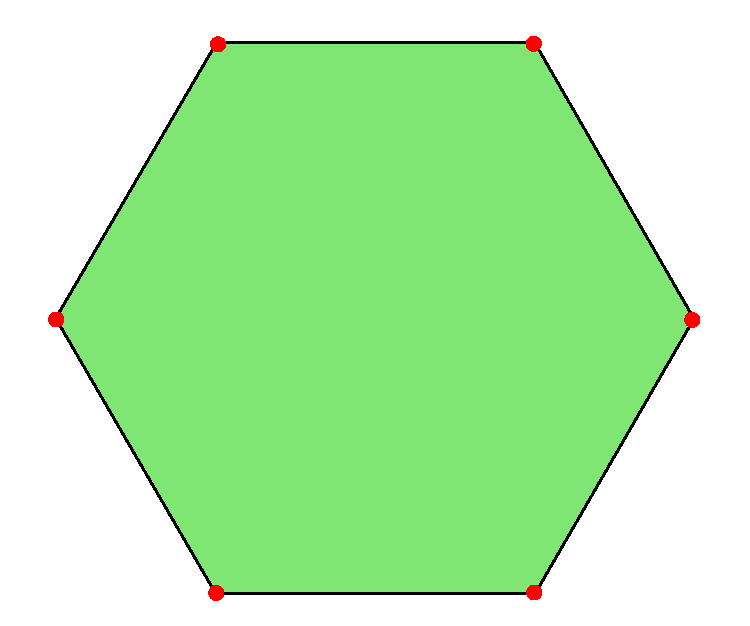
\includegraphics[width=1in]{../figures/hexagon0.pdf}}
    % \caption{Type I:5 tetrahedra}
%%
\subfigure{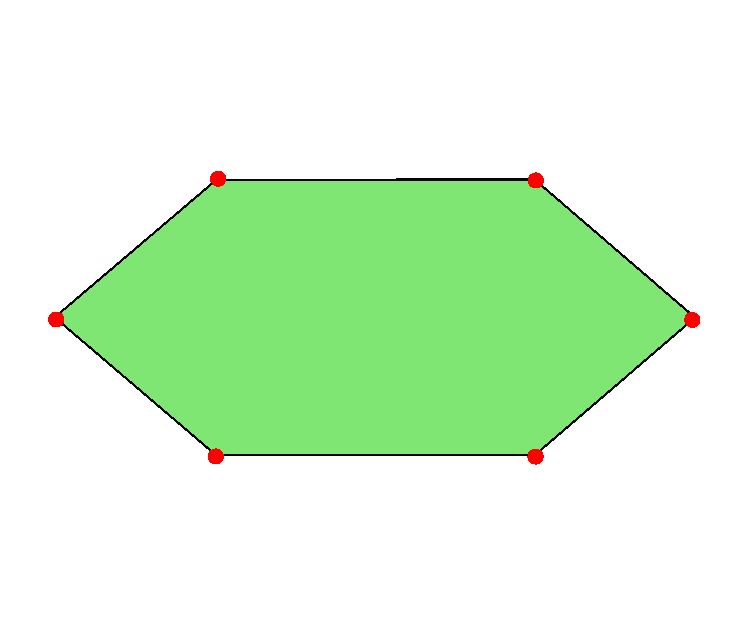
\includegraphics[width=1in]{../figures/hexagon3.pdf}}
     %\caption{Type II: 24 tetrahedra}
%%
\subfigure{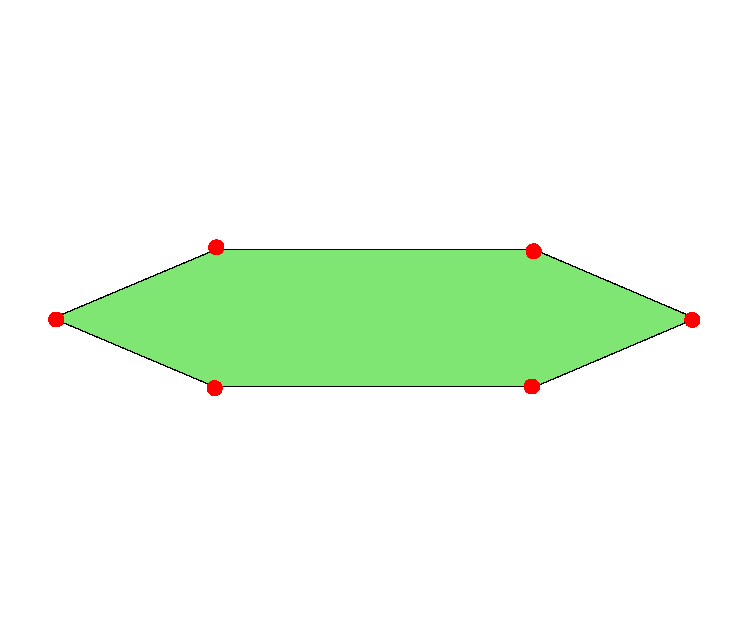
\includegraphics[width=1in]{../figures/hexagon4.pdf}}
     %\caption{Trirectangular tetrahedron}
%%
\caption{The hexagons $H_0, H_1, H_2$.}
  \label{fig:collapsehexagon} %% label for entire figure
\end{figure} 
We design two experiments to check the condition number of the stiffness
matrices of the four VEMs. 

Firstly, we refer to the ``collapsing polygons'' experiment in
\cite{Mascotto2018} and consider a sequence of hexagons
$\{H_i\}_{i=0}^{\infty}$, where the vertices of $H_i$ are given by
$A_i = (1, 0)$, $B_i = (0.5, a_i)$, $C_i = (-0.5, a)$, $D_i=(-1, 0)$, 
$E_i = (-0.5, -a_i)$, and $F_i = (0.5, -a_i)$,
where $a_i = \frac{\sqrt{3}}{2^{i+1}}$. The hexagons $H_0$, $H_1$ and $H_2$ are drawn
in Fig.~\ref{fig:collapsehexagon}. 
% We construct the virtual element space on $H_i$ and calculate the condition number
% of the stiffness matrix of four methods. 
As shown in Fig.~\ref{fig:collapsehexagon_conditionnumber} for $k=8$ and $k=10$, the condition numbers of stiffness
matrices of the stabilization-free methods are smaller than those of the standard methods when $i$ is large.

\begin{figure}[htbp]
\subfigure[$k = 8$]{
\begin{minipage}[t]{0.45\linewidth}
\centering
\includegraphics*[width=2in]{../figures/collapsing_condition_number_8.pdf}
\end{minipage}}%% 
\quad \quad
\subfigure[$k = 10$]
{\begin{minipage}[t]{0.45\linewidth}
\centering
\includegraphics*[width=2in]{../figures/collapsing_condition_number_10.pdf}
\end{minipage}}
\caption{The condition number of stiffness matrix of four VEMs on
$\{H_i\}_{i=0}^{12}$.}
\label{fig:collapsehexagon_conditionnumber}
\end{figure}

% \begin{figure}[htbp]
% \centering
% \subfigure{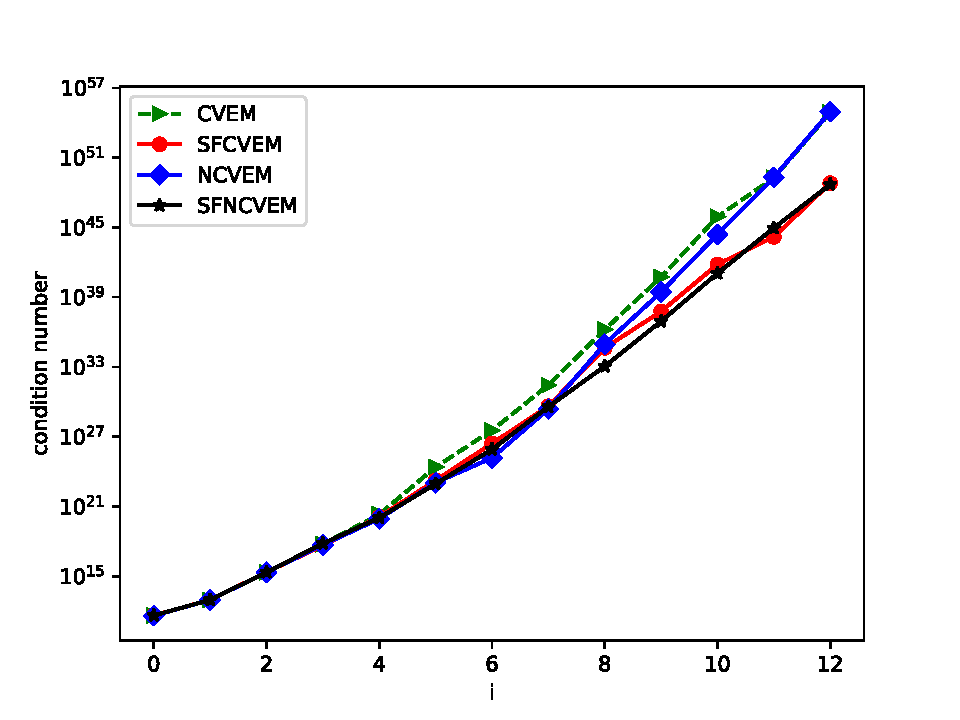
\includegraphics[width=2.2in]{./figures/collapsing_condition_number_8.pdf}}
% \subfigure{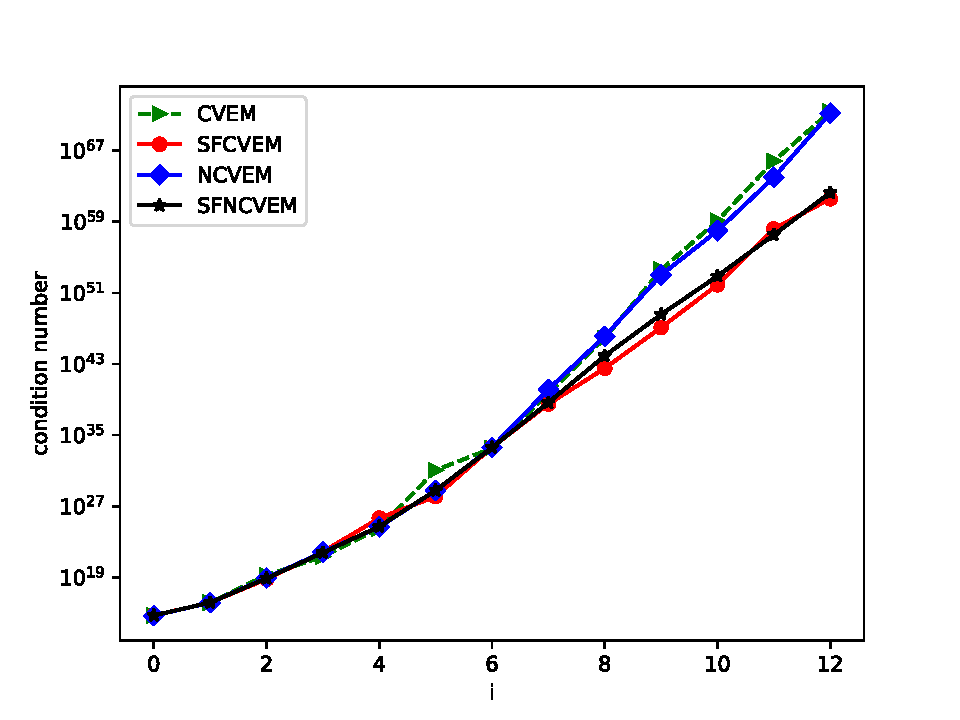
\includegraphics[width=2.2in]{./figures/collapsing_condition_number_10.pdf}}
% \caption{The condition number of stiffness matrix of four VEMs on
% $\{H_i\}_{i=0}^{12}$, Left : $k = 8$, Right : $k = 10$.}
%   \label{fig:collapsehexagon_conditionnumber0} %% label for entire figure
% \end{figure}

Secondly, we do the patch test for the Laplace equation with a nonhomogeneous Dirichlet boundary condition. Take the exact solution $u=1+x+y$. %We adopt meshes in Fig. \ref{fig:polymesh}.
% $$
% \left\{\begin{aligned}
% -\Delta u & = 0 \quad x \in \Omega\\
% u & = g \quad x \in \partial \Omega
% \end{aligned}\right.
% $$
% where $\Omega = (0, 1)^2, \ u = g = 1+x+y$. 
Let $h_x$ and $h_y$ be mesh size in the $x$-direction and
$y$-direction respectively.
We examine the behavior of error $\|u - u_h\|_0$ of the four VEMs in the
following three cases:
\begin{enumerate}[(1)]
\item Mesh in Fig.~\ref{fig:mesh}: Fix $h_x=h_y=0.2$ but vary $k= 1, 2, \ldots, 10$;
\item Mesh in Fig.~\ref{fig:mesh}: Fix $k=3$ but vary $h_x=h_y=2^{-i}$ for $i=1,\ldots, 5$;
\item Mesh in Fig.~\ref{fig:polymesh}: Fix $k=3$ and $h_x=0.2$, but vary $h_y=2^{-i}$ for $i=1,\ldots, 8$.
\end{enumerate}
\begin{figure}[htbp]
\centering
% \subfigure{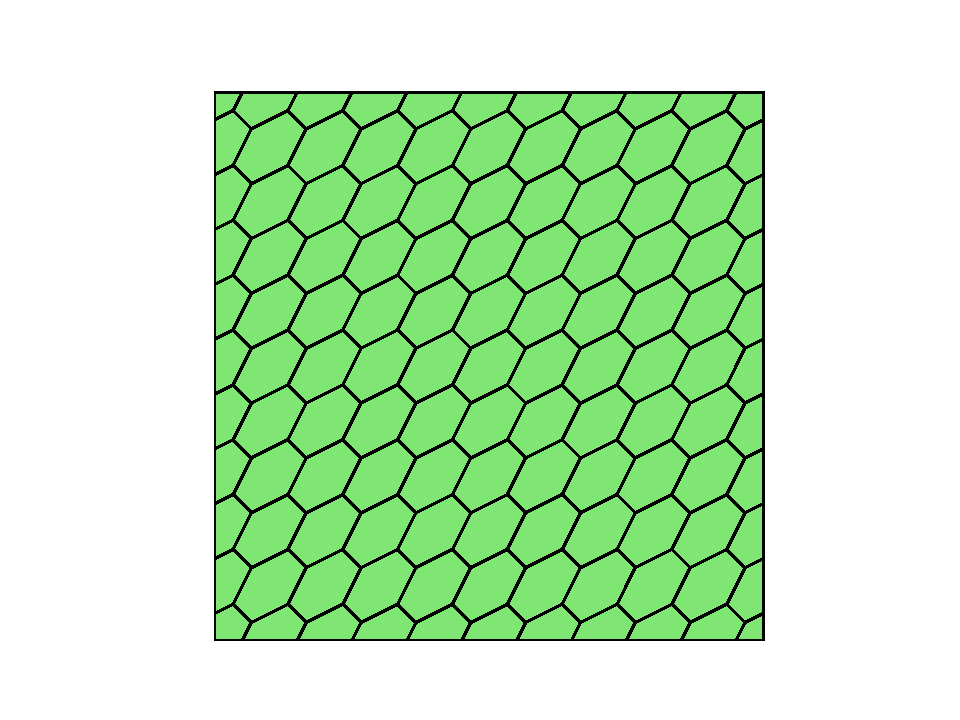
\includegraphics[width=2in]{./figures/poly_mesh.pdf}}
\subfigure{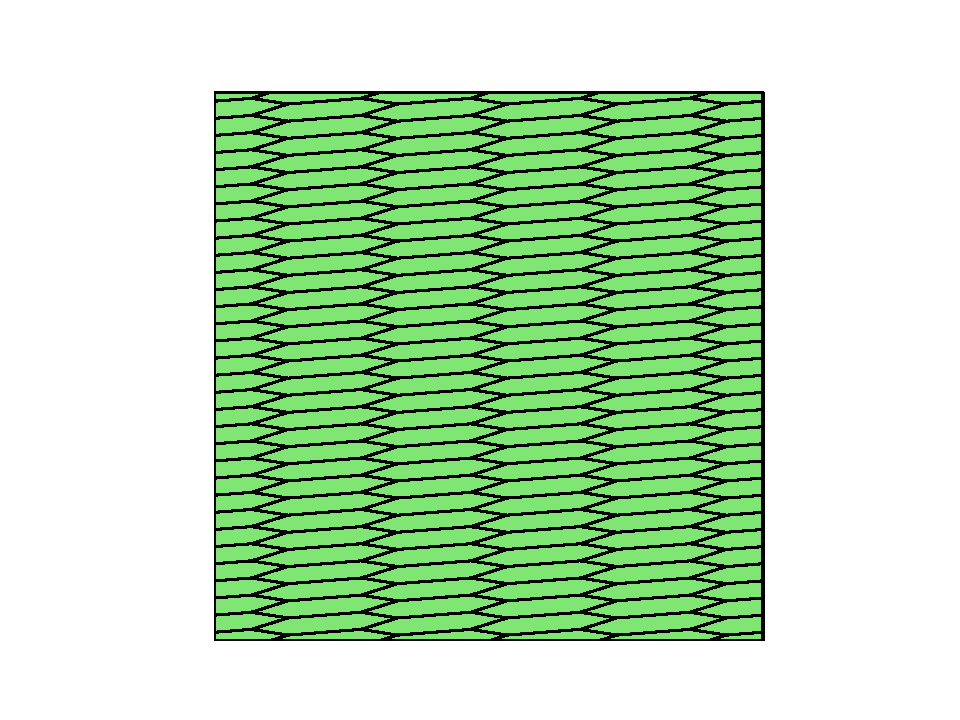
\includegraphics[width=2in]{../figures/mesh_hy.pdf}}
\caption{The mesh of domain $(0, 1)\times(0, 1)$ with
$h_x=0.2, h_y = 0.03125$.}
% \caption{The meshes of domain $(0, 1)\times(0, 1)$. Left: $h = 0.1$. Right:
% $h_x=0.2, h_y = 0.03125$.}
  \label{fig:polymesh} %% label for entire figure
\end{figure}
The errors of the four methods shown in Fig.~\ref{fig:patchtest} are similar. 
Since the error in the patch test
grows as the condition number of the stiffness matrix grows, 
the condition numbers of the stiffness matrix obtained by
four methods are comparable.
\begin{figure}[htbp]
\centering
\subfigure{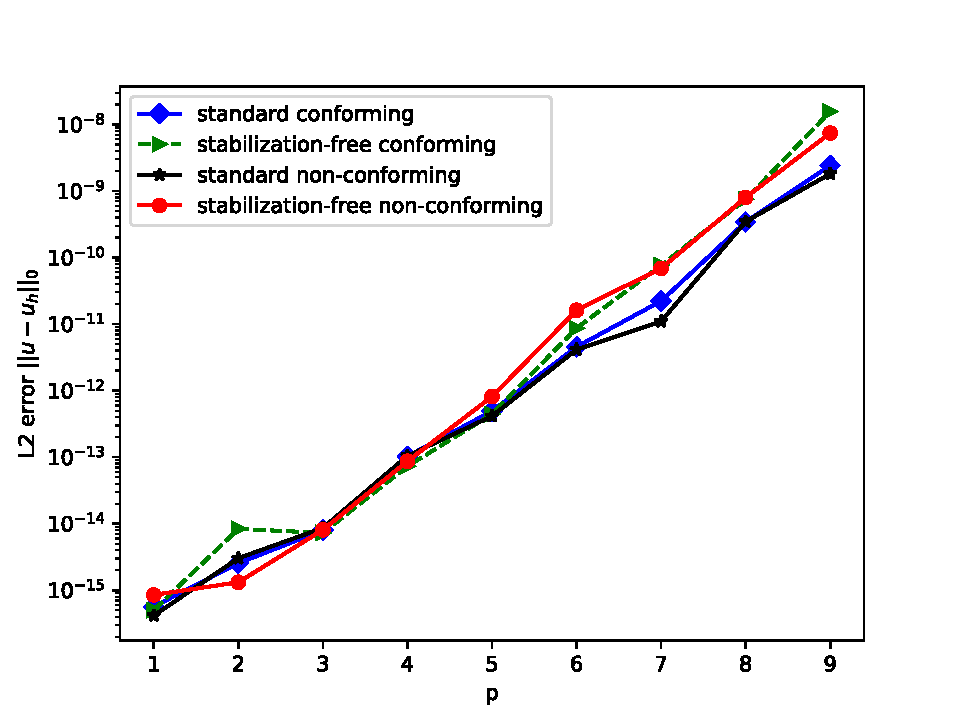
\includegraphics[width=1.7in]{../figures/patch_test_p.pdf}}
%%
\subfigure{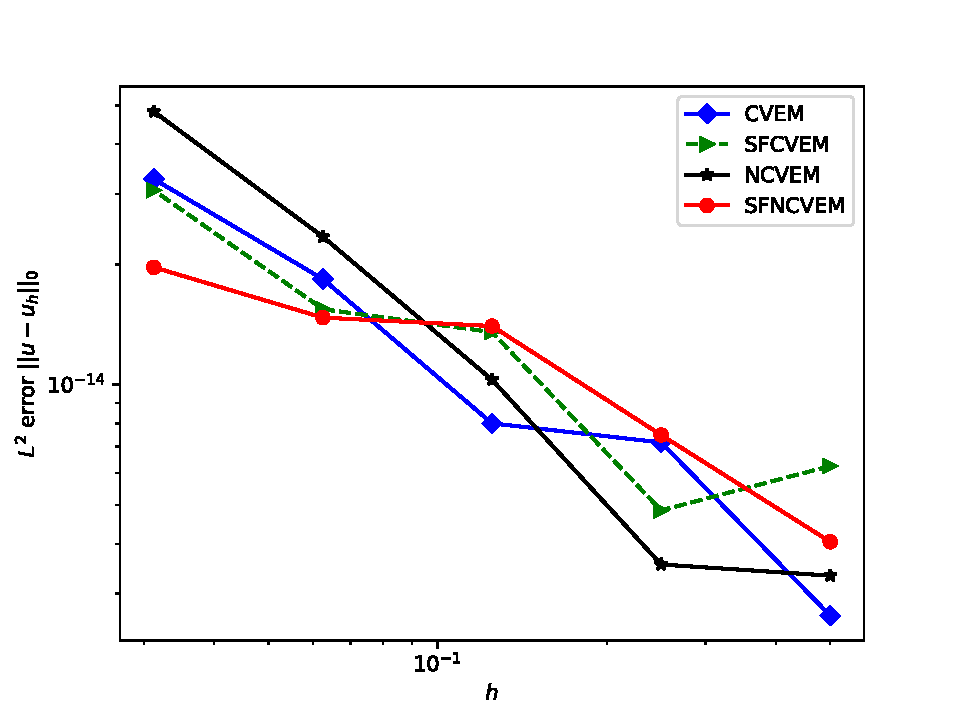
\includegraphics[width=1.7in]{../figures/patch_test_h.pdf}}
%%
\subfigure{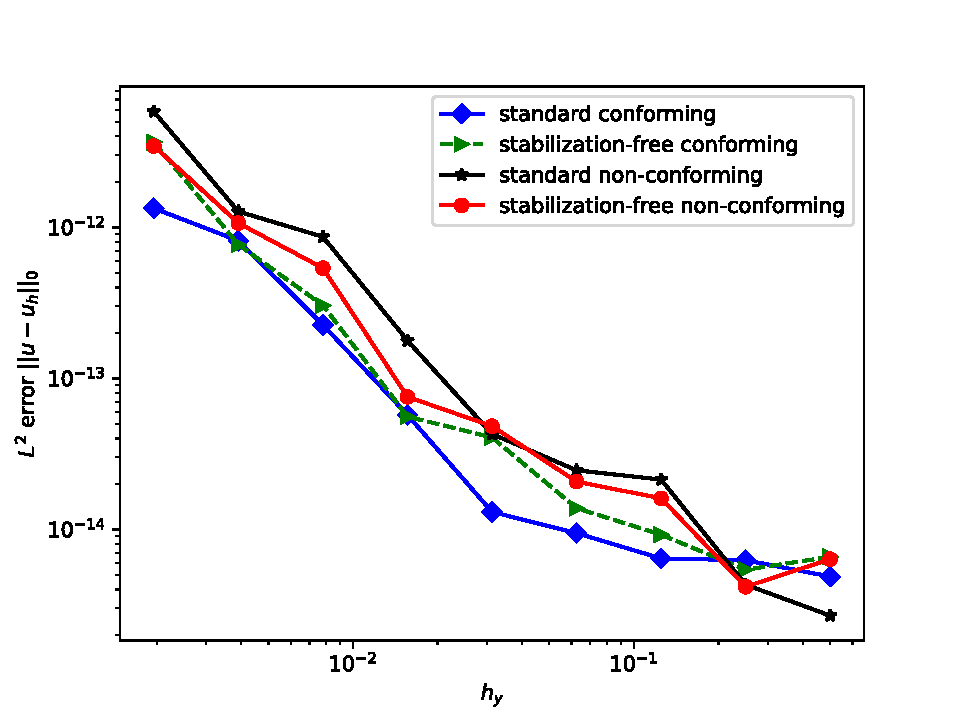
\includegraphics[width=1.7in]{../figures/patch_test_hy.pdf}}
\caption{The $L^2$ error of patch test.}
  \label{fig:patchtest} %% label for entire figure
\end{figure}

\medskip

\item \textsf{Minor issues (I will not highlight all the typos but only few of them as an example):
\begin{itemize}
\item line 3; “Poisson”$-\!\!\!-\!\!\!>$“the Poisson”;
\item line 24; “space”$-\!\!\!-\!\!\!>$“the space”;
\item line 31; “space”$-\!\!\!-\!\!\!>$“that the space”;
\item line 43; “usual”$-\!\!\!-\!\!\!>$“the usual”;
\item line 49; “space”$-\!\!\!-\!\!\!>$“the space”;
\item line 68; “. And”$-\!\!\!-\!\!\!>$“and”;
\item line 81; “banach”$-\!\!\!-\!\!\!>$“Banach”;
\item line 82; “and $\mathbb K$, where $\mathbb K$”$-\!\!\!-\!\!\!>$“and $\mathbb K$”; 
\item line 105; “surface”$-\!\!\!-\!\!\!>$“the surface”;
\item line 107; “smooth”$-\!\!\!-\!\!\!>$“a smooth”;
\item line 262; “shape”$-\!\!\!-\!\!\!>$“the shape”;
\item line 347; “discrete”$-\!\!\!-\!\!\!>$“the discrete”;
\item lines 465-466; “DoF”$-\!\!\!-\!\!\!>$“DoFs”; “is”$-\!\!\!-\!\!\!>$“are”; “vanishes”$-\!\!\!-\!\!\!>$“vanish”; 
\item line 511; “inequlities”$-\!\!\!-\!\!\!>$“inequalities”;
\item line 549; “DoFs”$-\!\!\!-\!\!\!>$“the DoFs”.
\end{itemize}
}

\smallskip \noindent \textcolor[rgb]{1.00,0.00,0.00}{Reply.}
We proofread the paper carefully. All of them have been corrected.


\end{enumerate}



\section{Response to Reviewer 2}
%\smallskip \noindent {\bf Response to Reviewer 2}.

\begin{enumerate}[1.]
\item \textsf{A significantly more thorough review of the literature is required. Indeed, very little mention of other stabilization free methods are given. It is difficult to gauge how this work compares to the existing literature and where the true novelty of the work lies. For example, in the reference \cite{CicuttinErnLemaire2019} a stabilisation free method is designed by considering a HHO space of unknowns and a reconstruction in a VEM space. See \cite[Remark 5.1]{CicuttinErnLemaire2019}. How does the current article compare to this work?}

\smallskip \noindent \textcolor[rgb]{1.00,0.00,0.00}{Reply.}
\begin{itemize}
    \item In addition to stabilization-free VEMs in \cite{BerroneBorioMarcon2021,BerroneBorioMarcon2022,DAltriMirandaPatrunoSacco2021,ChenSukumar2022,ChenSukumar2023,MengWangBuMei2022}, we add the reference \cite{CicuttinErnLemaire2019} for a stabilization-free hybrid high-order method, and the references
\cite{YeZhang2020,AlTaweelWang2020,AlTaweelWang2020a,YeZhang2021,YeZhang2021a,AlTaweelWangYeZhang2021} for stabilization-free weak Galerkin finite element methods.
    \item Next we compare the mixed-order HHO method in \cite{CicuttinErnLemaire2019} and the virtual element method. 

Recall the nonconforming virtual element in \cite{AyusodeDiosLipnikovManzini2016}.
The local virtual element space is
\[
W_k(K):=\{v\in H^1(K) : \Delta v\in\mathbb P_{k-2}(K),\, \partial_nv|_F\in\mathbb P_{k-1}(F)\textrm{ for }F\in\mathcal F(K)\}.
\]
The degrees of freedom are given by
\begin{align}
\frac{1}{|F|}(v, \phi_i^F)_F, & \quad i=1,\ldots, \dim\mathbb P_{k-1}(F), F\in\mathcal F(K), \label{eq:vemdof1}\\
\frac{1}{|K|}(v, \phi_i^K)_K, & \quad i=1,\ldots, \dim\mathbb P_{k-2}(K), \label{eq:vemdof2}
\end{align}
where $\{\phi_i^F\}_{i=1}^{\dim\mathbb P_{k-1}(F)}$ is a basis of $\mathbb P_{k-1}(F)$, and $\{\phi_i^K\}_{i=1}^{\dim\mathbb P_{k-2}(K)}$ a basis of $\mathbb P_{k-2}(K)$.
Then define the global virtual element space  
\begin{align*}
W_h&:=\{v_h\in L^2(\Omega): v_h|_K\in W_k(K) \textrm{ for each } K\in\mathcal T_h, \textrm{  } \\
&\qquad\; \textrm{DoFs \eqref{eq:vemdof1} are single-valued for $F\in\mathcal F_h$, and vanish for $F\in \mathcal F_h^{\partial}$}\}.
\end{align*}
By Remark 5.4 in \cite{CicuttinErnLemaire2019}, the mixed-order HHO method for the Poisson equation in~\cite{CicuttinErnLemaire2019} is equivalent to find $u_h\in W_h$ such that
\begin{equation}\label{eq:2023111}    
\sum_{K\in\mathcal T_h}(\nabla u_h, \nabla v_h)_K=\sum_{K\in\mathcal T_h}(f, Q_{k-2}^Kv_h)_K\quad\forall~v_h\in W_h.
\end{equation}
In Remark 5.1 in \cite{CicuttinErnLemaire2019}, the authors claim that the stabilization is no longer needed for the mixed-order HHO method, i.e. the method \eqref{eq:2023111}.
However, $(\nabla_h u_h, \nabla_h v_h)$ is not computable, % based on the degrees of freedom \eqref{eq:vemdof1}-\eqref{eq:vemdof2}, 
and the method \eqref{eq:2023111} is not the standard nonconforming VEM in \cite{AyusodeDiosLipnikovManzini2016}. 
% For the practical computation, a basis of $W_k(K)$ has to be solved approximately as shown in \cite[Remark 4.1]{CicuttinErnLemaire2019}. 
% The method \eqref{eq:2023111} is not the standard nonconforming virtual element method in \cite{AyusodeDiosLipnikovManzini2016}.
% However, the bilinear form $\displaystyle\sum_{K\in\mathcal T_h}(\nabla u_h, \nabla v_h)_K$ is not computable based on the degrees of freedom \eqref{eq:vemdof1}-\eqref{eq:vemdof2}, since some non-polynomial functions are included in the space $W_k(K)$.
For the practical computation, a basis of $W_k(K)$ has to be solved approximately as shown in 
Remark 4.1 in \cite{CicuttinErnLemaire2019}, which will always produce errors. 
When a basis of $W_k(K)$ is solved approximately (can't be solved exactly), the approximation of the space $W_h$ is no more a virtual element space, and the method \eqref{eq:2023111} is no more a virtual element method. See Remark 4.6.
\end{itemize}


\medskip

\item \textsf{Moreover, the authors do not make it clear what the benefit of a “stabilization-free” VEM is.}

\smallskip \noindent \textcolor[rgb]{1.00,0.00,0.00}{Reply.}
The stabilization term in virtual element methods (VEM) brings about some problems, which motivate us to develop stabilization-free VEMs. 
\begin{enumerate}
\item 
The local stabilization term $S_K(\cdot, \cdot)$ has to satisfy 
$$
c_{*} |v|_{1,K}^2\leq S_K(v,v)\leq c^{*} |v|_{1,K}^2 
$$
for $v$ belongs to the non-polynomial subspace of the virtual element space, which influences the condition number of the stiffness matrix and brings in the pollution factor $\frac{\max\{1, c^*\}}{\min\{1, c_*\}}$ in the error estimates \cite{DassiMascotto2018,BeiraodaVeigaDassiRusso2017,Mascotto2018}.  
\item 
The stabilization term appears in both side of the a posteriori error estimates when bounding the error by the residual error estimators \cite{CangianiGeorgoulisPryerSutton2017}.
\item 
For the a posteriori error analysis on anisotropic polygonal meshes in \cite{AntoniettiBerroneBorioDAuriaEtAl2022}, the stabilization dominates the error estimator, which makes the anisotropic a posteriori error estimator suboptimal. 
\item The stabilization term significantly affects the performance of the VEM for the Poisson eigenvalue problem \cite{BoffiGardiniGastaldi2020},
and improper choices of the stabilization term will produce useless results.
\item 
Special stabilization terms are designed for a nonlinear elasto-plastic deformation problem \cite{HudobivnikAldakheelWriggers2019} and an electromagnetic interface problem in three dimensions \cite{CaoChenGuo2023}, which are not easy to be extended to other problems.
\item Numerical examples in \cite{BerroneBorioMarcon2022} show that the stabilization-free VEM in \cite{BerroneBorioMarcon2021} outperforms the standard VEM in \cite{BeiraodaVeigaBrezziMariniRusso2016} for anisotropic elliptic problems on general convex polygonal meshes.
\end{enumerate}

\medskip

\item \textsf{At equation (3.4) (and continuing below) the space $\mathbb P_{k-2}(T;\mathbb K)\boldsymbol{x}$ is considered. Is this standard notation? At first I thought $\boldsymbol{x}$ was a predefined point (e.g. the centre of $T$) and the space $\mathbb P_{k-2}(T;\mathbb K)\boldsymbol{x}$ was the set of functions that could be written as a polynomial valued anti-symmetric tensor times the predefined point $\boldsymbol{x}$. However, I think what is actually meant is $\mathbb P_{k-2}(T;\mathbb K)\boldsymbol{x}=\{f:T\to\mathbb R^d: f(\boldsymbol{x})=\boldsymbol{P}_{k-2}(\boldsymbol{x})\boldsymbol{x},\quad \forall\boldsymbol{x}\in T, \boldsymbol{P}_{k-2}\in \mathbb P_{k-2}(T;\mathbb K)\}$. The authors should clarify here.}

\smallskip \noindent \textcolor[rgb]{1.00,0.00,0.00}{Reply.}
Yes, the notation $\mathbb P_{k-2}(T;\mathbb K)\boldsymbol{x}$ means
$$
\mathbb P_{k-2}(T;\mathbb K)\boldsymbol{x}:=\{\boldsymbol{\tau}\boldsymbol{x}: \boldsymbol{\tau}\in \mathbb P_{k-2}(T;\mathbb K)\},
$$
where $\boldsymbol{\tau}\boldsymbol{x}$ is the product of the matrix $\boldsymbol{\tau}$ and the independent variable $\boldsymbol{x}\in T$. Similar notations are used in \cite{ChenHuang2021divdiv,Chen;Huang:2020Finite}. In the revised manuscript, we define the notation $\mathbb P_{k-3}(T;\mathbb K)\boldsymbol{x}$ below DoFs (3.1)-(3.3).

\medskip

\item \textsf{Line 149: “$(I +\boldsymbol{x}\cdot\nabla)\boldsymbol{w} = \boldsymbol{0}$, which implies $\boldsymbol{w} = \boldsymbol{0}$”. I do not see how this follows. We have that
$$(\nabla\boldsymbol{w}(\boldsymbol{x}))\boldsymbol{x}=-\boldsymbol{w}(\boldsymbol{x})\quad\forall\boldsymbol{x}\in T.
$$
It is not clear to me how the conclusion that $\boldsymbol{w} = \boldsymbol{0}$ follows. The authors
should precise their reasoning.}

\smallskip \noindent \textcolor[rgb]{1.00,0.00,0.00}{Reply.}
The fact “$(I +\boldsymbol{x}\cdot\nabla)\boldsymbol{w} = \boldsymbol{0}$, which implies $\boldsymbol{w} = \boldsymbol{0}$” follows from \cite[(35)]{Chen;Huang:2020Finite}
%Recall (35) in \cite{Chen;Huang:2020Finite} that
\begin{equation}\label{eq:20230205}
\mathbb P_{k}(T)\cap\ker(I+\boldsymbol{x}\cdot\nabla)=\{0\}.
\end{equation}
Indeed, \eqref{eq:20230205} is a direct result of the Euler's formula \cite[(2.1)]{ChenHuang2021divdiv}
$$
\boldsymbol{x}\cdot\nabla q=kq\quad\forall~q\in \mathbb H_k(T),
$$
where $\mathbb H_k(T)$ is the space of homogeneous polynomials of degree $k$.

\medskip

\item \textsf{In the proof of Lemma 3.12, the authors apply a discrete trace inequality to the
quantity 
$$
\sum_{F\in\mathcal F^{\partial}(\mathcal T_K)}h_F^{1/2}\|\boldsymbol{\phi}\cdot\boldsymbol{n}\|_{0,F}
$$
and cite [11, (2.18)]. However, [11, (2.18)] is a continuous trace inequality and there is no justification given for why the discrete trace inequality holds in this particular case. Moreover, it is not explained how one concludes that $\|\div\boldsymbol{\phi}\|_{-1,K}\lesssim \|\boldsymbol{\phi}\|_{0,K}$.}

\smallskip \noindent \textcolor[rgb]{1.00,0.00,0.00}{Reply.}
For $F\in\mathcal F^{\partial}(\mathcal T_K)$, there exists a simplex $T\in\mathcal T_K$ satisfying $F\subset\partial T$. We can use the trace inequality \cite[(2.18)]{BrennerSung2018} and the inverse inequality to get
$$
h_F^{1/2}\|\boldsymbol{\phi}\cdot\boldsymbol{n}\|_{0,F} \lesssim \|\boldsymbol{\phi}\|_{0,T}+h_T|\boldsymbol{\phi}|_{1,T}\lesssim \|\boldsymbol{\phi}\|_{0,T}.
$$ 
Then
$$
\sum_{F\in\mathcal F^{\partial}(\mathcal T_K)}h_F^{1/2}\|\boldsymbol{\phi}\cdot\boldsymbol{n}\|_{0,F} \lesssim \sum_{F\in\mathcal F^{\partial}(\mathcal T_K)}\|\boldsymbol{\phi}\|_{0,T}\lesssim \|\boldsymbol{\phi}\|_{0,K}.
$$ 

For the second question, it can be explained as follows:
$$
\|\div\boldsymbol{\phi}\|_{-1,K}=\sup_{v\in H_0^1(K)}\frac{(\div\boldsymbol{\phi}, v)_K}{|v|_{1,K}}=-\sup_{v\in H_0^1(K)}\frac{(\boldsymbol{\phi}, \nabla v)_K}{|v|_{1,K}} \leq \|\boldsymbol{\phi}\|_{0,K}.
$$

\medskip

\item \textsf{In the proof of Lemma 4.1, the authors claim that
$$
h_K^{\frac{1}{2}}\|\partial_nv\|_{0,\partial K}\lesssim |v|_{1,K}.
$$
This is a sort of discrete trace inequality and the authors justify it by citing (A.3)-(A.4) in [15]. However, it is not apparent to me how this follows from (A.3)-(A.4). Moreover, the authors conclude that “with the multiplicative trace inequality”
$$
h_K^{\frac{1}{2}}\|v\|_{0,\partial K}\lesssim h_K^{-1}\|v\|_{0,K}.
$$
Again, this is a discrete trace inequality, and it is not specified why it is valid on the virtual space $V_k(K)$. The same goes for the arguments used in the proof of Lemma 4.3.}

\smallskip \noindent \textcolor[rgb]{1.00,0.00,0.00}{Reply.}
% One reviewer suggests removing the proof of Lemma 4.1, as it is standard in the virtual element literature. We agree with his suggestion, so we remove the proof of Lemma 4.1 in the revised manuscript. But we explain this comment in detail, and provide a complete proof of Lemma 4.1 here. 
\begin{itemize}
    \item 
For virtual function $v\in V_k(K)$, apply (A.3) in \cite{ChenHuang2020ncvem} to get
\[
h_K\|\Delta v\|_{0,K}\lesssim |v|_{1,K}.
\]
By (A.4) with $m=j=1$ in \cite{ChenHuang2020ncvem}, it follows that
\[
h_K^{1/2}\|\partial_nv\|_{0,\partial K}\lesssim |v|_{1,K}+h_K\|\Delta v\|_{0,K}.
\]
Combining the last two inequalities yields
\[
h_K\|\Delta v\|_{0,K}+h_K^{1/2}\|\partial_nv\|_{0,\partial K}\lesssim |v|_{1,K}.
\]
\item The multiplicative trace inequality is
\[
\|v\|_{0,\partial K}\lesssim h_K^{-1/2}\|v\|_{0,K}^{1/2}(\|v\|_{0,K}^{1/2}+h_K^{1/2}|v|_{1,K}^{1/2}) \quad\forall~v\in H^1(K).
\]
Since $v\in V_k(K)\subset H^1(K)$, inserting the last multiplicative trace inequality into the inequality
\[
|v|_{1,K}\lesssim h_K^{-1}\|v\|_{0,K}+h_K^{-1/2}\|v\|_{0,\partial K},
\]
we get
\begin{align*}
|v|_{1,K}&\lesssim h_K^{-1}\|v\|_{0,K}+h_K^{-1}\|v\|_{0,K}^{1/2}(\|v\|_{0,K}^{1/2}+h_K^{1/2}|v|_{1,K}^{1/2}) \\
&\lesssim h_K^{-1}\|v\|_{0,K}+h_K^{-1/2}\|v\|_{0,K}^{1/2}|v|_{1,K}^{1/2}.
\end{align*}
Then apply the Young's inequality to acquire the inverse inequality
\begin{equation*}%\label{eq:veminverse}
|v|_{1,K}\lesssim h_K^{-1}\|v\|_{0,K}\quad\forall~v\in V_k(K).  
\end{equation*}
\end{itemize}

% \vskip0.2cm
% \noindent\textcolor{cyan}{The complete proof of the inverse inequality \eqref{eq:veminverse} (i.e. Lemma 4.1) is given as follows.}
% \vskip0.2cm

% By (A.4) with $m=j=1$ in \cite{ChenHuang2020ncvem}, it follows that
% \[
% h_K^{1/2}\|\partial_nv\|_{0,\partial K}\lesssim |v|_{1,K}+h_K\|\Delta v\|_{0,K}.
% \]
% Then apply (A.3) in \cite{ChenHuang2020ncvem} to get
% \[
% h_K\|\Delta v\|_{0,K}+h_K^{1/2}\|\partial_nv\|_{0,\partial K}\lesssim |v|_{1,K}+h_K\|\Delta v\|_{0,K}\lesssim |v|_{1,K}.
% \]
% Employing the integration by parts and the Cauchy-Schwarz inequality, we have
% \[
% |v|_{1,K}^2=-(\Delta v,v)_K+(\partial_nv,v)_{\partial K}\leq\|\Delta v\|_{0,K}\|v\|_{0,K}+\|\partial_nv\|_{0,\partial K}\|v\|_{0,\partial K}.
% \]
% Combining the last two inequalities gives
% \[
% |v|_{1,K}\lesssim h_K^{-1}\|v\|_{0,K}+h_K^{-1/2}\|v\|_{0,\partial K},
% \]
% which together with the multiplicative trace inequality and the Young's inequality yields the inverse inequality \eqref{eq:veminverse}.


\medskip

\item \textsf{When introducing the nonconforming virtual element method in Section 4, the authors should give some references for NCVEM. In particular, I don’t think the space $V_k(K)$ is the classical NCVEM space (e.g. that defined in \cite{AyusodeDiosLipnikovManzini2016}). The authors should give reference to where this space is first introduced.}

\smallskip \noindent \textcolor[rgb]{1.00,0.00,0.00}{Reply.}
Thanks for this suggestion. We have revised the statement as follows:
Several $H^1$-nonconforming virtual elements are developed in \cite{AyusodeDiosLipnikovManzini2016,CangianiManziniSutton2017,ChenHuang2020ncvem,Huang2020}.
In this paper we adopt those in \cite{CangianiManziniSutton2017,ChenHuang2020ncvem}.

\medskip

\item \textsf{It seems that the main novelty of this work is the construction of a space
\begin{align*}
\mathbb V_{k-1}^{\div}(K):=\{\boldsymbol{\phi}&\in L^2(K): \div\boldsymbol{\phi}\in\mathbb P_{k-2}(K), \\
& \boldsymbol{\phi}\cdot\boldsymbol{n}_F\in\mathbb P^{k-1}(F)\;\forall F\in\mathcal F(K), \boldsymbol{\phi}|_T\in\mathbb P_{k-1}(T)^d\;\forall T\in\mathcal T_K
\}
\end{align*}
and a computable $L^2$ projector $Q_{K,k-1}^{\div}$ onto $\mathbb V_{k-1}^{\div}(K)$ such that
$$
\|Q_{K,k-1}^{\div}\nabla v\|_{0,K}\simeq \|\nabla v\|_{0,K} \quad\forall v\in V_k(K),
$$
where $V_k(K)$ is the non-conforming space defined at line 378 (or in Section 5 the authors consider the conforming space defined at line 544). This result is stated in Lemma 4.4 and its proof relies on the norm equivalence (3.32) and the set of uni-solvent DOFs (3.29)-(3.31). However, upon reading Section 3.2 for the first time, it is difficult to grasp what it is the authors are actually trying to achieve. Are all of the spaces, definitions and lemmas in Section 3.2 really necessary to prove Lemma 4.4? If so, the authors should state the main result of Lemma 4.4 in an earlier section, and leave much of the details of Section 3.2 and the proof of Lemma 4.4 to a later section so that readers can understand what the authors are trying to achieve.}

\smallskip \noindent \textcolor[rgb]{1.00,0.00,0.00}{Reply.}
Thanks for this nice suggestion. We add the following paragraph in the beginning of Section 3.

In this section we will construct an $H(\div)$-conforming macro finite element space $\mathbb{V}_{k-1}^{\rm div}(K)$ and the corresponding degrees of freedoms in arbitrary dimension, and establish the $L^2$ norm equivalence for $\boldsymbol{\phi}\in\mathbb{V}_{k-1}^{\rm div}(K)$
\begin{equation*}%\label{eq:Vkm1divnormequiv}
\|\boldsymbol{\phi}\|_{0,K}\eqsim h_K\|\div\boldsymbol{\phi}\|_{0,K} + \sup_{\boldsymbol{\psi}\in\div\mathring{\boldsymbol{V}}_{k}^{d-2}(K)}\frac{(\boldsymbol{\phi}, \boldsymbol{\psi})_K}{\|\boldsymbol{\psi}\|_{0,K}} +\sum_{F\in\mathcal F(K)}h_F^{1/2}\|\boldsymbol{\phi}\cdot\boldsymbol{n}\|_{0,F}.
\end{equation*}
The space $\mathbb{V}_{k-1}^{\rm div}(K)$ and its $L^2$ norm equivalence will be used to prove
the norm equivalence for the virtual element space
\begin{equation*}%\label{intro:gradVknormequiv} 
\|Q_{K,k-1}^{\div}\nabla v\|_{0,K}\eqsim \|\nabla v\|_{0,K} \quad \forall~v\in V_k(K),
\end{equation*}
where $V_k(K)$ is the nonconforming virtual element space in Section 4, and the conforming virtual element space in Section 5. Here $Q_{K,k-1}^{\div}$ is the computable $L^2$ projector onto the space $\mathbb{V}_{k-1}^{\rm div}(K)$.


\medskip

\item \textsf{In Section 4, the authors design a stabilization free NCVEM for a reaction-diffusion problem, and in section 5 a stabilization free VEM. This seems an odd choice as one does not require a Poincar\'e inequality for the coercivity of the continuous bilinear form. Indeed, if
$$
a(u, v)=(\nabla u, \nabla v)_{\Omega}+\alpha (u, v)_{\Omega}
$$
with $\alpha > 0$ then it holds trivially that
$$
\|u\|_{1,\Omega}^2\leq\max(1,\alpha^{-1})a(u,u).
$$
While things mightn't be so simple at the discrete level, it would seem more
appropriate to consider a Poisson problem.}

\smallskip \noindent \textcolor[rgb]{1.00,0.00,0.00}{Reply.} 
In this paper, we consider the reaction-diffusion problem with the homogeneous Dirichlet boundary condition. The Poincar\'e inequality is required for the coercivity of the bilinear form. In the continuous level, by the Poincar\'e inequality, we have the coercivity
\[
\|u\|_{1,\Omega}^2\lesssim |u|_{1,\Omega}^2\leq a(u,u)\quad \forall~u\in H_0^1(\Omega).
\]

The discrete bilinear form of the stabilization-free NCVEM in this paper is defined as 
\[
a_h(u_h, v_h):=(Q_{h,k-1}^{\div}\nabla_h u_h, Q_{h,k-1}^{\div}\nabla_h v_h)+\alpha(Q_hu_h, Q_hv_h).
\]
The discrete Poincar\'e inequality established in \cite{Brenner2003} works for the virtual element space $V_h$
\[
\|v_h\|_0\lesssim |v_h|_{1,h}\quad\forall~v_h\in V_h.
\]
This means that $|\cdot|_{1,h}$ is indeed a norm for space $V_h$. Hence, to show the coercivity of the discrete bilinear form $a_h(\cdot, \cdot)$, it suffices to prove
\begin{equation}\label{eq:11}    
|v_h|_{1,h}^2\lesssim a_h(v_h, v_h)\quad\forall~v_h\in V_h.
\end{equation}
The coercivity \eqref{eq:11} is (4.20) for the nonconforming virtual element method.
%, and~(5.8) for the conforming virtual element method.


\medskip

\item \textsf{In the numerical section, the authors should compare their results to standard VEM and NCVEM to highlight any benefit their approach has.}

\smallskip \noindent \textcolor[rgb]{1.00,0.00,0.00}{Reply.}
In the revised manuscript, we have provided many numerical experiments to compare our virtual element methods to the standard VEM and NCVEM. We also explain the benefit of the stabilization-free VEMs in the first paragraph in the introduction.

\medskip

\item \textsf{I suggest the authors conduct a thorough proof read of the manuscript as there are many typos, grammatical errors and poorly constructed sentences.}

\smallskip \noindent \textcolor[rgb]{1.00,0.00,0.00}{Reply.}
We try our best to proofread the manuscript carefully.




\end{enumerate}


\section{Response to Reviewer 3}
%\smallskip \noindent {\bf Response to Reviewer 2}.

\begin{enumerate}[1.]
\item \textsf{The paper under review presents an interesting and promising idea to avoid the stabilization term in the Virtual Element Method. The procedure adopted is very general and in principle can be used in many different settings. The paper is well written and the proofs are given with appropriate details. 
The only modification I require is a more in-depth comparison with the classical stabilized version with respect to the computational cost, in the two- and three-dimensional case, by making explicit examples in cases of interest.}

\smallskip \noindent \textcolor[rgb]{1.00,0.00,0.00}{Reply.}
In the revised manuscript, we have provided many numerical experiments to compare our virtual element methods to the classical stabilized VEMs in two dimensions. The comparison in three dimensions will be presented in future work.



\end{enumerate}


\bibliographystyle{abbrv}
\bibliography{../paper}

% ----------------------------------------------------------------
\end{document}
% ----------------------------------------------------------------
